In this notebook, you'll build a GAN using convolutional layers in the
generator and discriminator. This is called a Deep Convolutional GAN, or
DCGAN for short. The DCGAN architecture was first explored in 2016 and
has seen impressive results in generating new images; you can read the
\href{https://arxiv.org/pdf/1511.06434.pdf}{original paper, here}. \newline

You'll be training DCGAN on the
\href{https://www.cs.toronto.edu/~kriz/cifar.html}{CIFAR10} dataset.
These are color images of different classes, such as airplanes, dogs or
trucks. This dataset is much more complex and diverse than the MNIST
dataset and justifies the use of the DCGAN architecture.

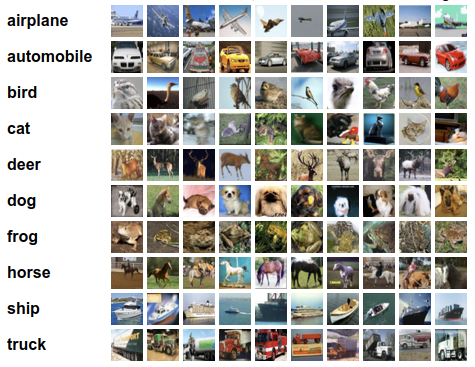
\includegraphics[width=1\linewidth]{img//genAdvNet//deepGAN/cifar10_data.png}

So, our goal is to create a DCGAN that can generate new,
realistic-looking images. We'll go through the following steps to do
this: 
\begin{itemize}
    \item Load in and pre-process the CIFAR10 dataset
    \item \textbf{Define discriminator and generator networks}
    \item Train these adversarial networks
    \item Visualize the loss over time and some sample, generated images
\end{itemize}

In this notebook, we will focus on defining the networks.

\paragraph{Deeper Convolutional Networks}

Since this dataset is more complex than our MNIST data, we'll need a
deeper network to accurately identify patterns in these images and be
able to generate new ones. Specifically, we'll use a series of
convolutional or transpose convolutional layers in the discriminator and
generator. It's also necessary to use batch normalization to get these
convolutional networks to train.\newline

Besides these changes in network structure, training the discriminator
and generator networks should be the same as before. That is, the
discriminator will alternate training on real and fake (generated)
images, and the generator will aim to trick the discriminator into
thinking that its generated images are real!

\subsection{Discriminator}

Here you'll build the discriminator. This is a convolutional classifier
like you've built before, only without any maxpooling layers. 
\begin{itemize}
    \item The inputs to the discriminator are 32x32x3 tensor images
    \item You'll want a few convolutional, hidden layers
    \item Then a fully connected layer for the output; as before, we want a sigmoid output, but we'll add that in the loss function, \href{https://pytorch.org/docs/stable/nn.html\#bcewithlogitsloss}{BCEWithLogitsLoss}, later
\end{itemize}

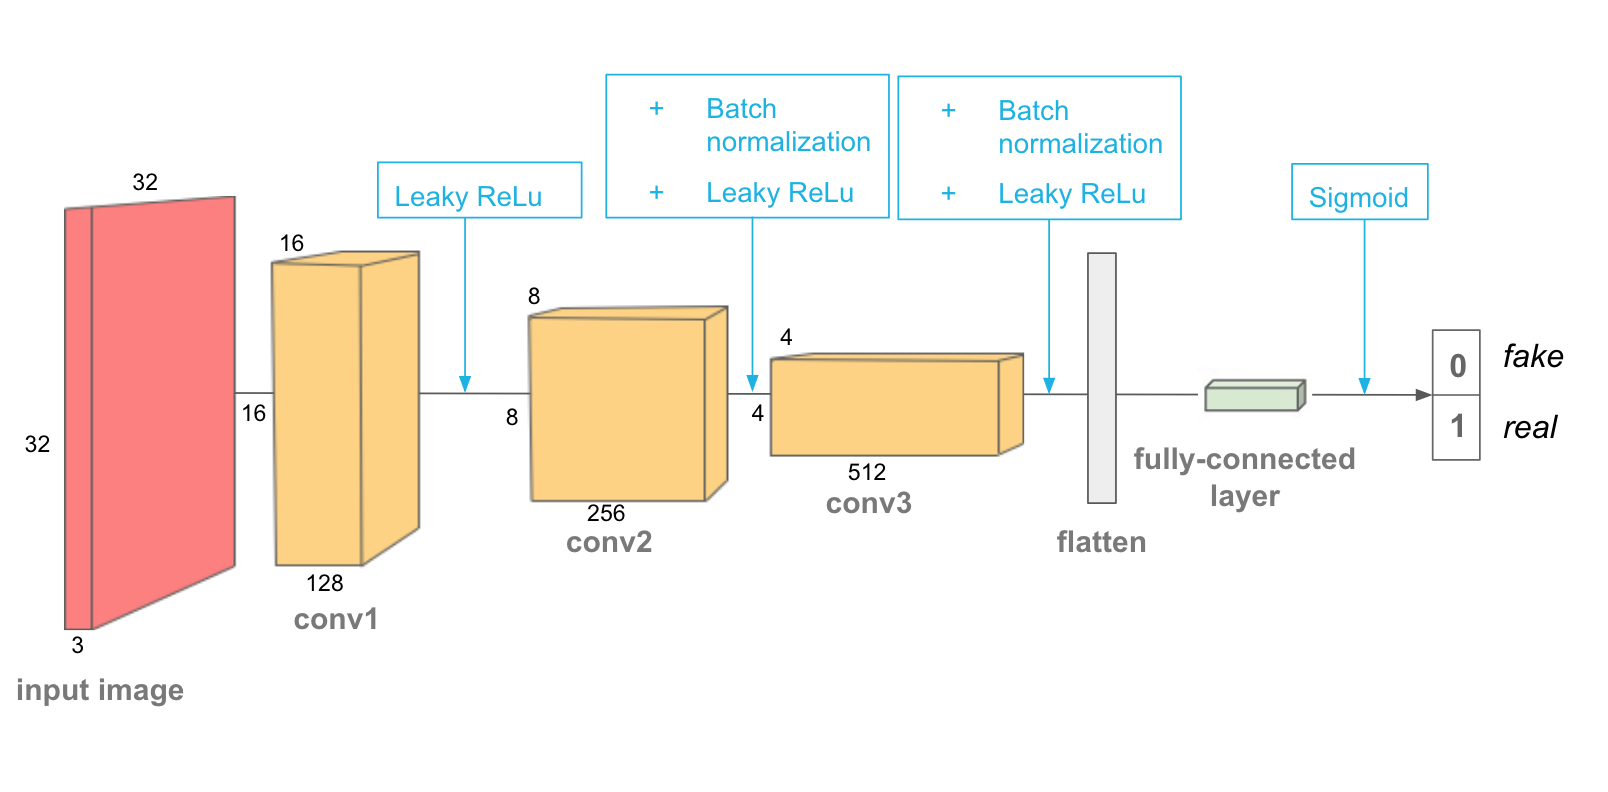
\includegraphics[width=1\linewidth]{img//genAdvNet//deepGAN/conv_discriminator.png}

For the depths of the convolutional layers I suggest starting with 32
filters in the first layer, then double that depth as you add layers (to
64, 128, etc.). Note that in the DCGAN paper, they did all the
downsampling using only strided convolutional layers with no maxpooling
layers. \newline

You'll also want to use batch normalization with
\href{https://pytorch.org/docs/stable/nn.html\#batchnorm2d}{nn.BatchNorm2d}
on each layer \textbf{except} the first convolutional layer and final,
linear output layer.

\paragraph{\texorpdfstring{Helper \texttt{ConvBlock}
module}{Helper ConvBlock module}}

In general, each layer should look something like convolution
\textgreater{} batch norm \textgreater{} leaky ReLU, and so we'll define
a \textbf{custom torch Module} to put these layers together. This module
will create a sequential series of a convolutional + an optional batch
norm layer.\newline

Note: It is also suggested that you use a \textbf{kernel\_size of 4} and
a \textbf{stride of 2} for strided convolutions.

\subsubsection{First exercise}

Implement the \lstinline{ConvBlock} module below and use
it for your implementation of the
\lstinline{Discriminator} module. Your discriminator
should take a 32x32x3 image as input and output a single logit.

\begin{lstlisting}[language=Python]
import torch
import torch.nn as nn

import tests
\end{lstlisting}

\begin{lstlisting}[language=Python]
class ConvBlock(nn.Module):
    """
    A convolutional block is made of 3 layers: Conv -> BatchNorm -> Activation.
    args:
    - in_channels: number of channels in the input to the conv layer
    - out_channels: number of filters in the conv layer
    - kernel_size: filter dimension of the conv layer
    - batch_norm: whether to use batch norm or not
    """
    def __init__(self, in_channels: int, out_channels: int, kernel_size: int, batch_norm: bool = True):
        super(ConvBlock, self).__init__()
        self.conv = nn.Conv2d(in_channels=in_channels, 
                              out_channels=out_channels, 
                              kernel_size=kernel_size, 
                              stride=2, 
                              padding=1,
                              bias=False)
        self.activation = nn.LeakyReLU(negative_slope=0.2)
        self.is_batch_norm = batch_norm
        self.bn = nn.BatchNorm2d(out_channels)
        
    def forward(self, x: torch.Tensor) -> torch.Tensor:
        x = self.conv(x)
        if self.is_batch_norm:
            x = self.bn(x)
        x = self.activation(x)
        return x
\end{lstlisting}

\begin{lstlisting}[language=Python]
class Discriminator(nn.Module):
    """
    The discriminator model adapted from the DCGAN paper. It should only contains a few layers.
    args:
    - conv_dim: control the number of filters
    """
    def __init__(self, conv_dim: int):
        super(Discriminator, self).__init__()
        self.conv_dim = conv_dim
        
        # input: 32x32, 1st layer no batch norm
        self.conv1 = ConvBlock(in_channels=3, 
                               out_channels=self.conv_dim, 
                               kernel_size=4, 
                               batch_norm = False)
        # input: 16x16
        self.conv2 = ConvBlock(in_channels=self.conv_dim, 
                               out_channels=self.conv_dim*2, 
                               kernel_size=4)
        # input: 8 x 8
        self.conv3 = ConvBlock(in_channels=self.conv_dim*2, 
                               out_channels=self.conv_dim*4, 
                               kernel_size=4)
        # output: 4x4
        
        # flatten
        self.flatten = nn.Flatten()
        # fully connected layer
        self.fcl = nn.Linear(conv_dim*4*4*4, 1) # self.conv_dimx4 (from the out channel) x 4 x 4
    def forward(self, x):
        x = self.conv1(x)
        x = self.conv2(x)
        x = self.conv3(x)
        x = self.flatten(x)
        x = self.fcl(x)  
        return x
\end{lstlisting}

\begin{lstlisting}[language=Python]
discriminator = Discriminator(64)
print(discriminator)
\end{lstlisting}

\begin{lstlisting}
Discriminator(
  (conv1): ConvBlock(
    (conv): Conv2d(3, 64, kernel_size=(4, 4), stride=(2, 2), padding=(1, 1), bias=False)
    (activation): LeakyReLU(negative_slope=0.2)
    (bn): BatchNorm2d(64, eps=1e-05, momentum=0.1, affine=True, track_running_stats=True)
  )
  (conv2): ConvBlock(
    (conv): Conv2d(64, 128, kernel_size=(4, 4), stride=(2, 2), padding=(1, 1), bias=False)
    (activation): LeakyReLU(negative_slope=0.2)
    (bn): BatchNorm2d(128, eps=1e-05, momentum=0.1, affine=True, track_running_stats=True)
  )
  (conv3): ConvBlock(
    (conv): Conv2d(128, 256, kernel_size=(4, 4), stride=(2, 2), padding=(1, 1), bias=False)
    (activation): LeakyReLU(negative_slope=0.2)
    (bn): BatchNorm2d(256, eps=1e-05, momentum=0.1, affine=True, track_running_stats=True)
  )
  (flatten): Flatten(start_dim=1, end_dim=-1)
  (fcl): Linear(in_features=4096, out_features=1, bias=True)
)
\end{lstlisting}

\begin{lstlisting}[language=Python]
tests.check_discriminator(discriminator)
\end{lstlisting}

\begin{lstlisting}
Congrats, you successfully implemented your discriminator
\end{lstlisting}

\subsection{Generator}

Next, you'll build the generator network. The input will be our noise
vector \lstinline{z}, as before. And, the output will be a
\(tanh\) output, but this time with size 32x32 which is the size of our
CIFAR10 images.

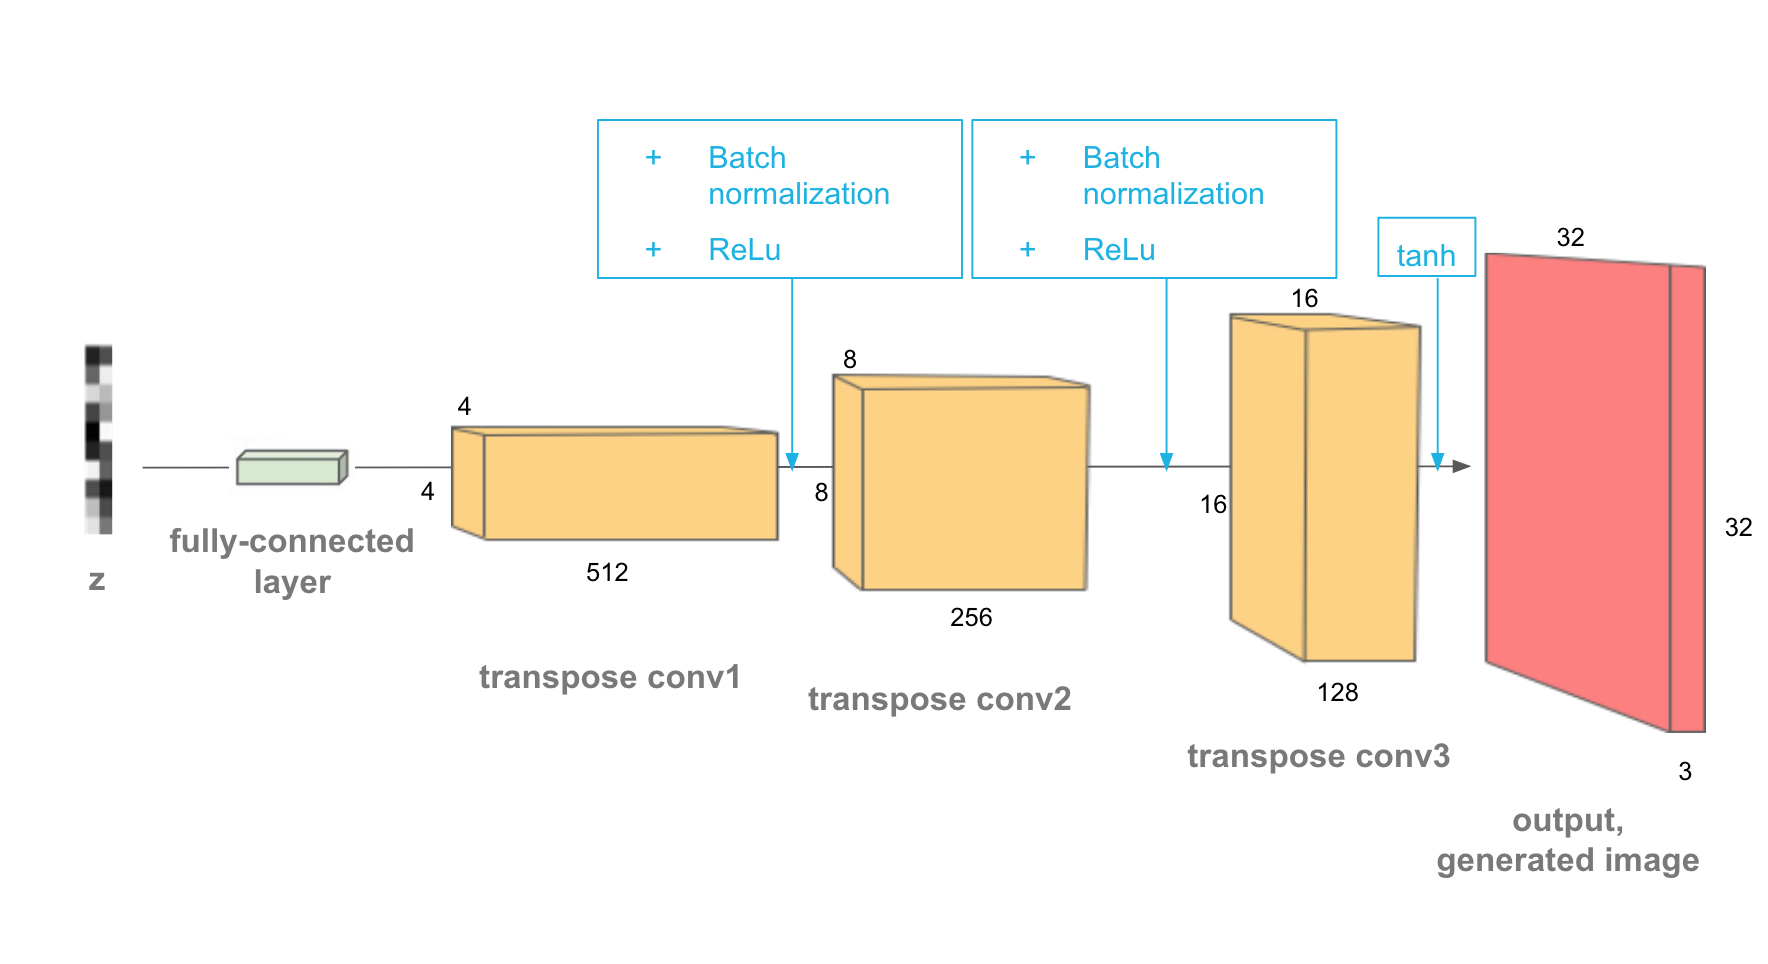
\includegraphics[width=1\linewidth]{img//genAdvNet//deepGAN/conv_generator.png}

What's new here is we'll use transpose convolutional layers to create
our new images. 
\begin{itemize}
    \item The first layer is a fully connected layer which is reshaped into a deep and narrow layer, something like 4x4x512.
    \item  Then, we use batch normalization and a leaky ReLU activation.
    \item Next is a series of \href{https://pytorch.org/docs/stable/nn.html\#convtranspose2d}{transpose convolutional layers}, where you typically halve the depth and double the width and height of the previous layer.
    \item And, we'll apply batch normalization and ReLU to all but the last of these hidden layers. Where we will just apply a \lstinline{tanh} activation.
\end{itemize}

\paragraph{\texorpdfstring{Helper \texttt{DeconvBlock}
module}{Helper DeconvBlock module}}

For each of these layers, the general scheme is transpose convolution
> batch norm > ReLU, and so we'll define a
function to put these layers together. This function will create a
sequential series of a transpose convolutional + an optional batch norm
layer. We'll create these using PyTorch's Sequential container, which
takes in a list of layers and creates layers according to the order that
they are passed in to the Sequential constructor.\newline

Note: It is also suggested that you use a \textbf{kernel\_size of 4} and
a \textbf{stride of 2} for transpose convolutions.

\paragraph{Second exercise}

Implement the \lstinline{DeconvBlock} module below and use
it for your implementation of the \lstinline{Generator}
module. Your generator should take a latent vector of dimension 128 as
input and output a 32x32x3 image.

\begin{lstlisting}[language=Python]
class DeconvBlock(nn.Module):
    """
    A "de-convolutional" block is made of 3 layers: ConvTranspose -> BatchNorm -> Activation.
    args:
    - in_channels: number of channels in the input to the conv layer
    - out_channels: number of filters in the conv layer
    - kernel_size: filter dimension of the conv layer
    - stride: stride of the conv layer
    - padding: padding of the conv layer
    - batch_norm: whether to use batch norm or not
    """
    def __init__(self, 
                 in_channels: int, 
                 out_channels: int, 
                 kernel_size: int, 
                 stride: int,
                 padding: int,
                 batch_norm: bool = True):
        super(DeconvBlock, self).__init__()
        self.tConv = nn.ConvTranspose2d(in_channels=in_channels,
                                         out_channels=out_channels, 
                                         kernel_size=kernel_size, 
                                         stride=stride, 
                                         padding=padding,
                                         bias=False)
        self.activation = nn.ReLU()
        self.bn = nn.BatchNorm2d(out_channels)
        self.batch_norm = batch_norm
        
    def forward(self, x: torch.Tensor) -> torch.Tensor:
        x = self.tConv(x)
        if self.batch_norm:
            x = self.bn(x)
        x = self.activation(x)
        return x
\end{lstlisting}

\begin{lstlisting}[language=Python]
class Generator(nn.Module):
    """
    The generator model adapted from DCGAN
    args:
    - latent_dim: dimension of the latent vector
    - conv_dim: control the number of filters in the convtranspose layers
    """
    def __init__(self, latent_dim: int, conv_dim: int = 32):
        super(Generator, self).__init__()
        self.latent_dim = latent_dim
        self.conv_dim = conv_dim
        self.layer1 = DeconvBlock(in_channels=self.latent_dim, 
                                  out_channels=self.conv_dim*4, 
                                  kernel_size=4, 
                                  stride=1, 
                                  padding=0)
        self.layer2 = DeconvBlock(in_channels=self.conv_dim*4, 
                                  out_channels=self.conv_dim*2, 
                                  kernel_size=4, 
                                  stride=2, 
                                  padding=1)
        self.layer3 = DeconvBlock(in_channels=self.conv_dim*2, 
                                  out_channels=self.conv_dim, 
                                  kernel_size=4, 
                                  stride=2, 
                                  padding=1)
        self.layer4 = nn.ConvTranspose2d(in_channels=self.conv_dim,
                                         out_channels=3, 
                                         kernel_size=4, 
                                         stride=2, 
                                         padding=1)
        self.last_activation = nn.Tanh()
        
    def forward(self, x):
        x = self.layer1(x)
        x = self.layer2(x)
        x = self.layer3(x)
        x = self.layer4(x)
        x = self.last_activation(x)
        return x
\end{lstlisting}

\begin{lstlisting}[language=Python]
generator = Generator(128)
print(generator)
\end{lstlisting}

\begin{lstlisting}
Generator(
  (layer1): DeconvBlock(
    (tConv): ConvTranspose2d(128, 128, kernel_size=(4, 4), stride=(1, 1), bias=False)
    (activation): ReLU()
    (bn): BatchNorm2d(128, eps=1e-05, momentum=0.1, affine=True, track_running_stats=True)
  )
  (layer2): DeconvBlock(
    (tConv): ConvTranspose2d(128, 64, kernel_size=(4, 4), stride=(2, 2), padding=(1, 1), bias=False)
    (activation): ReLU()
    (bn): BatchNorm2d(64, eps=1e-05, momentum=0.1, affine=True, track_running_stats=True)
  )
  (layer3): DeconvBlock(
    (tConv): ConvTranspose2d(64, 32, kernel_size=(4, 4), stride=(2, 2), padding=(1, 1), bias=False)
    (activation): ReLU()
    (bn): BatchNorm2d(32, eps=1e-05, momentum=0.1, affine=True, track_running_stats=True)
  )
  (layer4): ConvTranspose2d(32, 3, kernel_size=(4, 4), stride=(2, 2), padding=(1, 1), bias=False)
  (last_activation): Tanh()
)
\end{lstlisting}

\begin{lstlisting}[language=Python]
tests.check_generator(generator, 128)
\end{lstlisting}

\begin{lstlisting}
Congrats, you successfully implemented your discriminator
\end{lstlisting}
